%%%%%%%%%% NO OLVIDAR COLOCAR ESTE COMENTARIO CON EL NUMERO DE EJERCICIO %%%%%%%%%%%%%
%%%%%%%%%%%%%%%%%%% EJERCICIO 2 %%%%%%
%%Text bf para negrilla , el \\ es para el salto de linea.
%%El primer \\ hace un espacio en el texto y el 2 \\ crea otro espacio
\textbf{Ejemplo 2}\newline
El jefe de producción de una fábrica debe decidir entre dos máquinas A y B. Las características de cada una son: \\
\begin{center}
		\begin{tabular}{|p{1cm}|p{2cm}|p{2cm}|p{2cm}|p{3cm}|}
			\hline
			\rowcolor{white!50}
			\textbf{Maq.} & \textbf{C} & \textbf{K} & \textbf{S} & \textbf{CAO} \\ \hline
			A            & 800.000 COP   & 3 años     & 200.000 COP    & 25.000 COP       \\ \hline
			B            & 600.000 COP   & 2 años     & 150.000 COP    & 30.000 COP       \\ \hline
		\end{tabular}
\end{center}

Con una tasa del 36\% nominal anual año vencido, determinar la mejor alternativa.

\textbf{Solución.}\\
\begin{center}
	\renewcommand{\arraystretch}{1.5}% Margenes de las celdas
	%Creación de la cuadricula
	\begin{longtable}[H]{|c|c|c|}
		%Creamos una linea horizontal
		\hline
		%Definimos el color de la primera fila
		\rowcolor[HTML]{FFB183}
		%%%%% INICIO ASIGNACIÓN FECHA FOCAL %%%%%%%
		%%%%%%%%%% INICIO TITULO
		%Lo que se hace aquí es mezclar las 3 columnas en una sola
		\multicolumn{3}{|c|}{\cellcolor[HTML]{FFB183}\textbf{1. Asignación período focal}}   \\ \hline
		%%%%%%%%%% FIN TITULO
		%%%%% INICIO DECLARACIÓN DE VARIABLES %%%%%%%
		\multicolumn{3}{|c|}{$pf = 0  \textit{ pav }$} \\ \hline
		%Definimos el color de la primera fila
		\rowcolor[HTML]{FFB183}
		%%%%% INICIO DECLARACIÓN DE VARIABLES %%%%%%%
		%%%%%%%%%% INICIO TITULO
		\multicolumn{3}{|c|}{\cellcolor[HTML]{FFB183}\textbf{2. Declaración de variables}}                                                                                   \\ \hline
		%%%%%%%%%% FIN TITULO
		%%%%%%%%%% INICIO DE MATEMÁTICAS
		$\text{Alternativa A}$ & $\text{Alternativa B}$ & $i= 36\% \text{ pav }$\\
		$C =  800{.}000\text{ COP}$ & $C =  600{.}000\text{ COP}$ & $CPUE =  ?\text{ COP}$\\
		$K =  3 \textit{ años}$ & $K =  2 \textit{ años}$ & \\
		$S =  200{.}000\text{ COP}$ & $S =  150{.}000\text{ COP}$ & \\
		$CAO =  25{.}000\text{ COP}$ & $CAO =  30{.}000\text{ COP}$ & \\
 		$n_{1}= 3 \text{ pav}$ & $n_{2}= 2 \text{ pav}$ &   \\\hline 
		%%%%%%%%%% FIN DE MATEMÁTICAS
		%%%%% FIN DECLARACIÓN DE VARIABLES


		%%%%% INICIO FLUJO DE CAJA
		\rowcolor[HTML]{FFB183}
		\multicolumn{3}{|c|}{\cellcolor[HTML]{FFB183}\textbf{3. Diagrama de flujo de caja}}\\ \hline
		%Mezclamos 3 columnas y pondremos el dibujo
		%%%%%%%%%%%%% INSERCIÓN DE LA IMAGEN
		\multicolumn{3}{|c|}{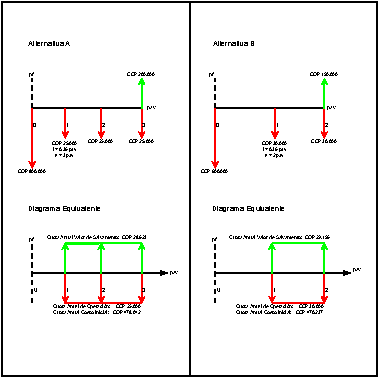
\includegraphics[trim=-5 -5 -5 -5 , scale=2]{10_Capitulo/ejemplos/2/Ejemplo_2.pdf}}
        \\\hline
		%%%%%%%%%%%%% FIN INSERCIÓN DE IMAGEN
		%%%%%FIN FLUJO DE CAJA



		%%%%% INICIO DECLARACIÓN FORMULAS
		%%%%%%%%%%% INICIO TITULO
		\rowcolor[HTML]{FFB183}
		\multicolumn{3}{|c|}{\cellcolor[HTML]{FFB183}\textbf{4. Declaración de fórmulas}} \\ \hline
		%%%%%%%%%%% FIN TITULO
		%%%%%%%%%%% INICIO MATEMÁTICAS

		\multicolumn{3}{|c|}{$VP=R\frac{1-(1+i_{1})^{-n}}{i_{2}} \text{ Valor presente serie uniforme vencida}$}\\ 
		\multicolumn{3}{|c|}{$VF=R\frac{1-(1+i_{1})^{n}}{i_{2}} \text{ Valor futuro aserie uniforme vencida}$}\\\hline
		%%%%%%%%%% FIN MATEMÁTICAS
		%%%%%% INICIO DESARROLLO MATEMÁTICO
		\rowcolor[HTML]{FFB183}
		%%%%%%%%%%INICIO TITULO
		\multicolumn{3}{|c|}{\cellcolor[HTML]{FFB183}\textbf{5. Desarrollo matemático}}   \\ \hline
		%%%%%%%%%% FIN TITULO
		%%%%%%%%%% INICIO MATEMÁTICAS
		Alternativa A & \multicolumn{2}{c|}{Alternativa B}\\ \hline
		Cuota anual costo inicial & \multicolumn{2}{c|}{Cuota anual costo inicial} \\
		${R=\frac{800{.}000}{\frac{1-(1,36)^{-3}}{0,36}} = 178{.}042}\text{ COP}$ & \multicolumn{2}{c|}{${R=\frac{600{.}000}{\frac{1-(1,36)^{-2}}{0,36}} = 470{.}237 }\text{ COP}$} \\
		Cuota anual valor salvamento & \multicolumn{2}{c|}{Cuota anual valor salvamento}\\
		$R=\frac{200{.}000}{\frac{(1,36)^{3}}{0,36}} = 28{.}623\text{ COP} $ & \multicolumn{2}{c|}{$R=\frac{150{.}000}{\frac{(1,36)^{2}}{0,36}} = 29{.}196 \text{ COP}$} \\
		CPUE alternativa A & \multicolumn{2}{c|}{CPUE alternativa B} \\ 
		$CPUE_{A} = 28.623-478.042-25.000 $ & \multicolumn{2}{c|}{$CPUE_{B} = 29.196-470.237-30.000$}\\ 
		$CPUE_{A} = -474.419\text{ COP}$ & \multicolumn{2}{c|}{$CPUE_{B} = -471.04$\text{ COP}}\\
		\hline
		%%%%%%%%%% FIN MATEMÁTICAS
		%%%%%% FIN DESARROLLO MATEMÁTICO

		\rowcolor[HTML]{FFB183}
		\multicolumn{3}{|c|}{\cellcolor[HTML]{FFB183}\textbf{6. Respuesta}}    \\ \hline

		\multicolumn{3}{|c|}{La alternativa que representa menores perdidad es la B.} \\ 
		\hline
	\end{longtable}
	%Se crean dos lineas en blanco para que no quede el siguiente texto tan pegado
	%\newline \newline
\end{center}
%%%%%%%%%%%%%%%%%%%%%%%%%%FIN EJERCICIO X %%%%%%%%%%%%%%%%%%%%%%%%%%%


